	\documentclass{article}
			
		\usepackage{parskip}
		\usepackage{listings}
		\usepackage{xcolor}
		\usepackage{textcomp}
			
		%STYLE AND COLOR DEFINITION FOR SOURCE CODE 	
		\newcommand{\PHPamountofcolor}{75}
		\newcommand{\SourceCodeContext}{5}
		%Lets define the php language colors:
		\definecolor{PHP_comment_old}{HTML}{FF8000}
		\colorlet{PHP_comment}{PHP_comment_old!\PHPamountofcolor!black}
		\definecolor{PHP_default_old}{HTML}{000000}
		\colorlet{PHP_default}{PHP_default_old!\PHPamountofcolor!black}
		\definecolor{PHP_keyword_old}{HTML}{6c9c11}
		\colorlet{PHP_keyword}{PHP_keyword_old!\PHPamountofcolor!black}
		\definecolor{PHP_emph1_old}{HTML}{0F58A2}
		\colorlet{PHP_emph1}{PHP_emph1_old!\PHPamountofcolor!black}
		\definecolor{PHP_emph2_old}{HTML}{CCAA00}
		\colorlet{PHP_emph2}{PHP_emph2_old!\PHPamountofcolor!black}
		\definecolor{PHP_emph4_old}{HTML}{C60484}
		\colorlet{PHP_emph4}{PHP_emph4_old!\PHPamountofcolor!black}
		\definecolor{PHP_string_old}{HTML}{C78F0A}
		\colorlet{PHP_string}{PHP_string_old!\PHPamountofcolor!black}
		\definecolor{PHP_variable_old}{HTML}{C82210}%C82210
		\colorlet{PHP_variable}{PHP_variable_old!\PHPamountofcolor!black}
		\definecolor{PHP_number_old}{HTML}{BF1CA6}
		\colorlet{PHP_number}{PHP_number_old!\PHPamountofcolor!black}
		%Now we want to highlight the variables. This will be done by triggering the function \PHPhighlightvar at the start of any $ run. This function wil only highlight variables and any other identifiers will be ignored. Luckily lstlisting will only give correct identifiers so we only will have to check if the previous call was made with a $
		\usepackage{fontspec}
		\setmonofont{Courier}
		%\usepackage[utf8]{inputenc}
		%\usepackage[T1]{fontenc}
		%\usepackage{courier, textcomp}
		\usepackage{etoolbox}
		\newtoggle{InString}{}% Keep track of if we are within a string
		\togglefalse{InString}% Assume not initally in string
		
		\newcommand*{\ColorIfNotInString}[1]{\iftoggle{InString}{#1}{\color{PHP_number}#1}}%

		%helper
		
		\newcommand{\PHPhighlightvar}[1]{\ifnum\theDollarFlag=1 \color{PHP_variable} \fi#1\setcounter{DollarFlag}{0}}
		\newcounter{DollarFlag}
		
		%images
		\usepackage{graphicx}
		\graphicspath{ {images/} }
		\usepackage{wrapfig}
		\usepackage{subcaption}
		
		
			
			
			
		
			
			\title{Artificial Intelligence:  Homework on Planning}

			\author{Edoardo Ghini}
			
			\begin{document}
			
			\textbf{\maketitle}
			\pagenumbering{gobble}
			
			\bigskip\bigskip\bigskip
			\begin{center}
			
\includegraphics[width=0.5\textwidth]{laSapienza}
			\end{center}
			\bigskip\bigskip\bigskip
			\textbf{
			Dipartimento di Ingegneria dell'Università di Roma La Sapienza}
			

			\newpage
			\pagenumbering{roman}
			\tableofcontents
			\newpage
			\pagenumbering{arabic}
			
			
			
			
			
			%SETTING STYLE OF SOURCE CODE
			\lstset{
		  language        = php,
		  basicstyle      = \footnotesize\ttfamily,
		  keywordstyle    = \color{PHP_keyword},
		  stringstyle     = \color{PHP_string!90!black}\toggletrue{InString},
		  %this allows highlighting of variables:
		  literate        =  {\$}{{\iftoggle{InString}{\$}{\setcounter{DollarFlag}{1}\color{PHP_variable}\$\color{PHP_default}}}}1
		%    {"}{{{\ProcessQuote{"}}}}1% Disable coloring within double quotes
		%    {'}{{{\ProcessQuote{'}}}}1% Disable coloring within single quote
		    {0}{{{\ColorIfNotInString{0}}}}1
		    {1}{{{\ColorIfNotInString{1}}}}1
		    {2}{{{\ColorIfNotInString{2}}}}1
		    {3}{{{\ColorIfNotInString{3}}}}1
		    {4}{{{\ColorIfNotInString{4}}}}1
		    {5}{{{\ColorIfNotInString{5}}}}1
		    {6}{{{\ColorIfNotInString{6}}}}1
		    {7}{{{\ColorIfNotInString{7}}}}1
		    {8}{{{\ColorIfNotInString{8}}}}1
		    {9}{{{\ColorIfNotInString{9}}}}1,
		  identifierstyle = \color{PHP_default}\PHPhighlightvar,
		  commentstyle    = \color{PHP_comment}\slshape,
		  emph            =[1]{require_once, require, include_once, include, namespace, use, class, function, new},
		  emphstyle       =[1]\color{PHP_emph1},%\bf,
		  emph            =[2]{echo, empty, isset, array, instanceof},
		  emphstyle       =[2]\color{PHP_emph2},%\bf,
		  emph            =[3]{var, const, abstract, 
		                        protected, private, public,
		                        static, final, extends, implements,
		                        global, if, else, foreach ,for,
		                        endforeach, endif, endfor, elseif,
		                        as},
		  emphstyle       =[3]\color{PHP_keyword},%\bf,
		  emph            =[4]{return, throw, exit, __halt_compiler, continue, break},
		  emphstyle       =[4]\color{PHP_emph4},%\bf,
		  breaklines      = true,
		  captionpos      = b,
		  rulecolor       =\color{black},
		  keywords    ={__halt_compiler,    abstract,   and,    array,
		                    as, break,  callable,   case,   catch,  class,
		                    clone,  const,  continue,   declare,    default,
		                    die,    do, echo,   else,   elseif,
		                    empty,  enddeclare, endfor, endforeach, endif,
		                    endswitch,  endwhile,   eval,   exit,   extends,
		                    final,  finally,    for,    foreach,    function,
		                    global, goto, if,   implements, include,
		                    include_once,   instanceof, insteadof,
		                    interface,  isset, list,    namespace,
		                    new,    or, print, private, protected,  public,
		                    require,    require_once, return,   static,
		                    switch, throw,  trait, try, unset, use, var,
		                    while,  xor,    yield,
		  },
		  numbers=left,
		  stepnumber=1,  
		  numberfirstline=true,
		  numberstyle=\footnotesize,
		  xleftmargin=4.0ex,
		  upquote=true,
		  showlines=true
		  }	
			
			\renewcommand{\lstlistingname}{Code}

			
			\part{Introduction}
			
			The most important factor that deserves to be taken into consideration approaching to a logic based problem is, certainly, the capability to represent the problem through a coherent domain abstraction.\smallskip\\
This essential concept is at base of which I am going to debate.\\
In fact, there will be the application of the planning techniques like fast-forward planning, partial ordering and hierarchical planning, on an abstract model built onto a real world problem.

\newpage
			\part{Development}
				\section{Vanilla Grid}
				At first the model has been built according to a simplification of the problem : a robot has to navigate through a gris world from a start position to the goal position. It would have to find the path toward the solution avoiding possible walls.
				\subsection{Strips formulation}

In order to obtain a representation which could bring to a resolution of the problem I used the formalism of STRIPS.  
				\subsubsection{Predicates}
			
				\begin{lstlisting}[caption= vanilla grid predicates, label=vanpred]
	connected( square-1  square-2)
	white ( square)
	black ( square)
	at ( who where)
	place ( where )
\end{lstlisting}
				\subsubsection{Actions}
				Accordingly with the extreme minimality of the domain, only one action has been enough to be able to create a successfull plan
 							\begin{lstlisting}[caption= vanilla grid actions, label=vanact]
Action: Move( who, from, to ) 
	Precondition: 
		At( who, from ),
                  place ( from),
                  place ( to),
                  connected ( from, to),
                  white( to)
         Effect:
                  at ( who to),
              	� at (who from)
                  
\end{lstlisting}
				
				\subsubsection{Initial and goal states}
		\begin{lstlisting}[caption= vanilla goal and initial state, label=vinigoal]
Initial State:
	place( square0-0) ^ place( square0-1) ^ place( square1-0) ^ place( square1-1) ^ ...
...	connected( square0-0 square 0-1) ^ connected( square0-0 square1-0)  ^ ...
...	black( square0-0) ^ black(square 0-1) ^ black( square1-0) ^ white( square1-1) ^ ...
...	at( robot square1-1)
Goal State:
	at( robot square10-1)
\end{lstlisting}
				About the initial configuration,  I defined every single square of the grid and also each link of reachability between each other and also the fact that there where white squares that correspond to the floor of the house and, similarly black cells that stand for walls.
				\subsection{Planner result}
				
				In fig(1), it cold be seen the path found from the planner in order to satisfy the goal precondition.
\begin{center}	
\begin{figure}
\centering
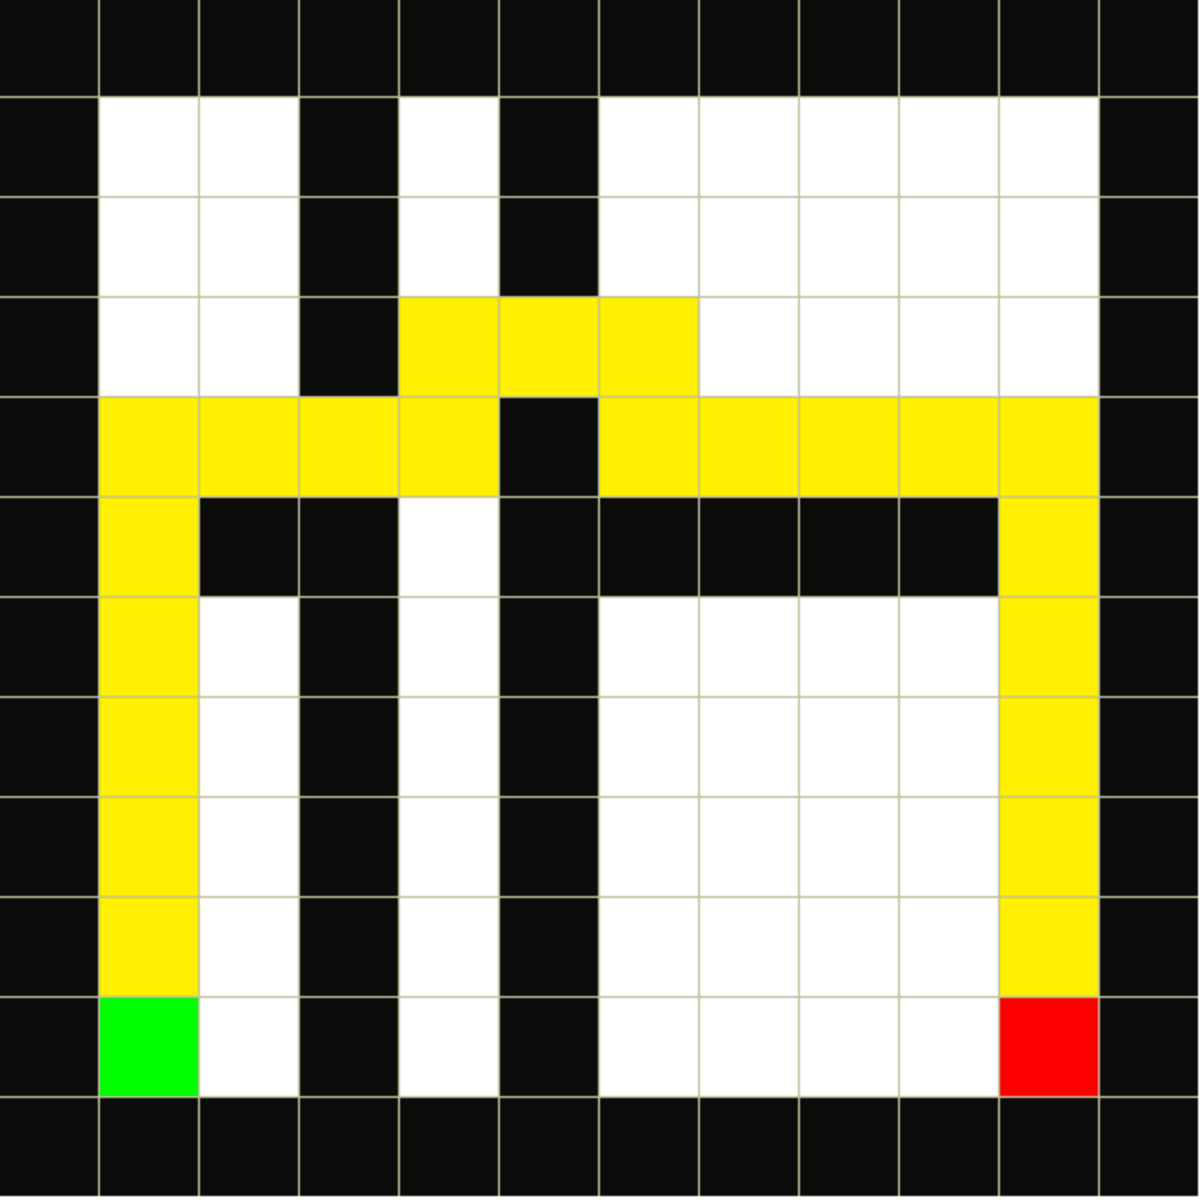
\includegraphics[width=0.5\textwidth]{van-final}
\caption{}
\label{fig:1}
\end{figure}
\end{center}

\newpage


				\section{Extended Grid}
				For the purpose of obtaining a more complex domain, the real world has changed and other objects and properties have been added.
				
				\subsection{Strips formulation}
				In the same fashion as the vanilla problem, I designed a representation of the real world through predicates and actions.
				\subsubsection{Predicates}
				
				Unlike in PDDL, in STRIPS we can't explicitly express equality constraints and for this reason I have had to specify objects like seat and tray with unambiguous predicates.\smallskip\\
				In other words, I added redundancy to represent multiple similar objects in the model.
				\begin{lstlisting}[caption= extended grid predicates, label=exepred]
	carry ( who, what),
  	seat1 ( seat),
	seat2 ( seat),
  	table ( where),
  	robot ( who),
  	white ( where),
  	black ( where),
  	closet ( where),
  	dishwasher ( where),
  	finished ( what),
  	washingmachine ( where),
	not-started-yet ( what),
  	clean ( what),
  	at ( who, where),
  	tray1 ( what),
	tray2 ( what),
	cloth ( what),
  	conn ( square-1 square-2),
  	unloaded ( who),
  	clear ( where)
\end{lstlisting}
			
				\subsubsection{Actions}
				\begin{lstlisting}[caption= exetended grid actions, label=exeact]
	
Action: Move( who, from, to)
    	 Precondition:
	 	robot ( who),
                 white ( from),
                 white ( to),
                 at ( who, from),
                 conn (from, to)
    	Effect:   
    		� at ( who, from),
                 at ( who, to)

Action: Put (who, what, where, near)
    Preconditions:
                 carry ( who, what),
                 white ( near),
                 at ( who, near),
                 conn ( near where)
    Effect:
    		unloaded ( who),
                 � carry ( who, what),
                 at ( what, where)
\end{lstlisting}
                  
                
                                   At a certain point, I thought that there would be some reasons to support the division of the run action in two sub-actions, allowing an easier management of the preconditions.\smallskip\\
                  In addition, during the definition of both the actions I needed to solve another problem: STRIPS language doesn't allow to define actions with negative preconditions.\\
                  Hence I introduced a dual predicate in order to use it in the preconditions in the place of the negated one. This was the case with not-started-yet( what) and finished (what).
                  \newpage
                  
                  \begin{lstlisting}[caption=extended grid run actions, label=exrunact]
                  
Action:  Run-washingmachine ( who, what, near, inside)
	Preconditions:
	 	robot ( who),
                 washingmachine ( what),
                 white ( near),
                 conn ( near, what),
                 at ( who, near),
                 not-started-yet ( what),
                 cloth ( inside),
                 at ( inside, what )
         Effect:
         	finished ( what),
                 clean ( inside),
                 � not-started-yet( what)
Action:   Run-dishwasher  ( who, what, near, inside1, inside2)
    	Precondition:
		robot ( who),
                 dishwasher ( what),
                 white ( near),
                 conn ( near, what),
                 at ( who, near),
                 not-started-yet ( what),
                 tray1 ( inside1),
                 at ( inside1, what),
                 tray2 ( inside2),
                 at ( inside2, what)
        Effect:        
    		finished ( what),
                 clean ( inside1),
                 clean ( inside2),
                  � not-started-yet( what)
                  
                  
\end{lstlisting}


                    Similarly as what I have done with run actions, I chose to divide the action take in four sub-actions and also I met the same problem as before: there was need of negative preconditions.\smallskip\\
                    In order to overcame this issue I have created another dual predicate, but this time the oldest ( loaded( who )  ) would have been substituted completely by  its logic negation : unloaded( who).
                  
                  	\begin{lstlisting}[caption= vanilla grid take actions, label=vanacttake]
Action: Take-cloth-from-table ( who, what, where, near, seat-1, seat-2)
    	Precondition:
		robot( who),
                 cloth ( what),
                 table ( where),
                 white ( near),
                 seat1( seat-1),
                 seat2 ( seat-2),
                 clear ( seat-1),
                 clear ( seat-2),
                 at ( who, near),
                 conn ( near, where),
                 at ( what, where),
                 unloaded ( who)
           Effect:
    		carry ( who, what),
                 � unloaded ( who),
                 � at( what where),
                 clear ( where)
                 
Action:  Take-tray-from-seat ( who, what, where, near )
      	   Precondition: 
	   	robot ( who),
                 tray ( what),
                 seat (where),
                 white ( near),
                 conn ( near, where),
                 at ( who, near),
                 at ( what, where),
                 unloaded ( who)
            Effect:
    		� unloaded ( who),
                 carry ( who, what),
                 � at ( what, where ),
                 clear ( where)
         
Action:  Take-cloth-from-waschingmachine ( who, what, where, near)
	Precondition:
    		robot ( who),
                 unloaded ( who),
                 cloth ( what),
                 washingmachine ( where),
                 white ( near),
                 conn ( near, where),
                 at ( who, near),
                 at ( what, where),
                 finished ( where)
    	Effect:
	 	 � unloaded ( who),
                  carry ( who, what),
                  � at ( what, where)
                  
Action:   Take-tray-from-dishwasher  (who, what, where, near)
  	Precondition:
		robot( who),
                 unloaded( who),
                 tray ( what),
                 dishwasher ( where),
                 white ( near),
                 conn ( near, where),
                 at ( who, near),
                 at ( what, where),
                 finished ( where)
	Effect:
  		� unloaded ( who),
                carry ( who, what),
                 � at ( what, where)
                 
\end{lstlisting}
               

                  
				\subsubsection{Initial and goal states}
				Likewise I have done in the simpler vanilla domain, I initialised the problem defining grid squares and their connections, objects positions and some predicates which where true from the beginning.\smallskip\\ Differently from vanilla world, there isn't the predicate ' place ( where) ' anymore because there where more specific places to model in the domain, for instance a table, two seats, a closet and so on and so forth.\smallskip\\
				In fig(2), there is a graphical representation of the model. 
				
				
				\begin{center}	
\begin{figure}
\centering
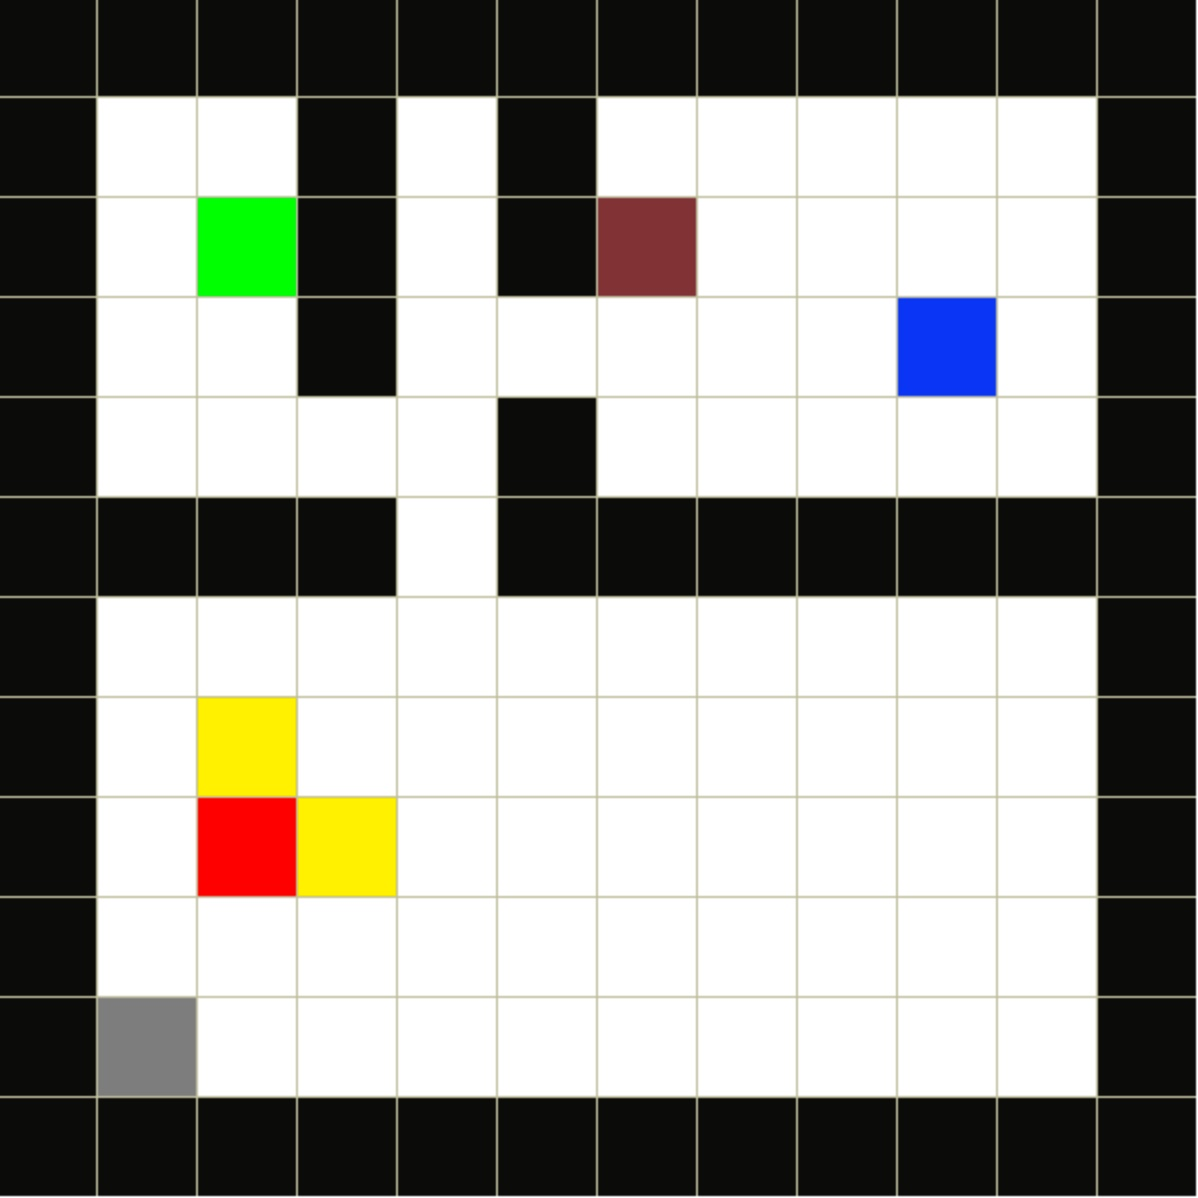
\includegraphics[width=0.5\textwidth]{exe-final}
\caption{}
\label{fig:2}
\end{figure}
\end{center}


				\begin{lstlisting}[caption= vanilla goal and initial state, label=vinigoal]
	Initial State:
		connected( square0-0 square 0-1) ^ connected( square0-0 square1-0)  ^ ...
	...	black( square0-0) ^ black(square 0-1) ^ black( square1-0) ^ white( square1-1) ^ ...
	...	at( robot1 square7-1) ^^ seat1( square3-3) ^ seat2( square2-4) ^ table( square2-3) ^
		^ dishwasher( square9-8) ^ washingmachine( square2-9) ^ closet( square6-9) ^
		^ tray1( tray-1) ^ at( tray-1 square3-3) ^ tray2( tray-2 square2-4) ^ cloth( cloth1) ^
		^ at( cloth1 node2-3) ^ robot( robot1) ^
		^ not-started-yet( square2-9) ^ not-started-yet( square9-8)
		
	Goal State:
		at( tray-1 square6-7) ^ at( tray-2 square6-9) ^ at( cloth1 square2-3) ^
		^ clean( tray-1) ^ clean( tray-2) ^ clean( tray-3)
\end{lstlisting}
				\subsection{Planner result}
				When the resolver tried to find a plan for this domain modelled in PDDL, he succeed without instantiating hard actions.\medskip\\
				Under those circumstances the search space will be smaller, hard actions should be avoided, consequently it is advisable to not introduce "or" clauses in the PDDL implementation.
				\begin{lstlisting}[caption= plan generated on extended grid, label=planex]
	
	0.77 seconds instantiating 6921932 easy, 0 hard action templates
               1.91 seconds reachability analysis, yielding 795 facts and 1216 actions
               0.00 seconds creating final representation with 502 relevant facts, 0 relevant fluents
               0.00 seconds computing LNF
               0.01 seconds building connectivity graph
               0.06 seconds searching, evaluating 744 states, to a max depth of 20
               2.75 seconds total time
\end{lstlisting}
\newpage

				\section{POP}
				Subsequently I simulated a partial order planning on the extended grid domain.
				\subsection{Design choices}
				I tried to be coherent with the STRIPS and PDDL formulation, in fact the graph can be seen as as a composition of three main threads which corresponds at three similar action sequences regarding the three object that are involved: two trays and one cloth. 
				\subsection{Abstraction level}
				One significative choice that i have made in order to simplify the domain was to consider the action move without preconditions.\smallskip\\ This, in fact, means that it could be executed at any time from any situations.
				\subsection{Conflict resolution}
				For this reason, an action move without precondition, the plan computation turned to be smooth because I did't meet conflicts of some sorts.\medskip\\
				But, at the same time, due to the fact that the robot could move in any situation toward anywhere, there are a lot of clubbering links between actions like put and take or also run and the single action move toward a different location.\medskip\\
				For instance I represented only one case of clubber presence in fig(3) with green arrows: the robot could decide to pursue another object in order to clean the house like the first tray or the closet if the first tray has already been taken instead of going on taking the just cleaned second tray.
				\newpage
				\subsection{Graph representation}
				In the afore mentioned fig(3) there is the graphical representation
\begin{center}	
\begin{figure}
\centering
\includegraphics[width=0.9\textwidth]{pop-ext}
\caption{}
\label{fig:3}
\end{figure}
\end{center}
\newpage
				\subsection{Plan order}
				It will follow the sequence of actions which I have computed during planning operations:\medskip\\
				Order -->  { MoveTo( robot table), Take( robot tray1), MoveTo( robot dishwasher), 
Put(robot tray1 dishwasher), MoveTo( robot table), Take (robot tray2), MoveTo( robot dishwasher), Put ( robot tray2 dishwasher), Rundishwasher(robot), MoveTo( robot table), Take( robot cloth), MoveTo(robot washingmachine), Put( robot cloth washingmachine), Runwashingmachine( robot), MoveTo( robot dishwasher), Take( robot Tray1), MoveTo(robot closet), Put (robot tray1 closet), MoveTo(robot dishwasher) ,Take (robot tray2), MoveTo(robot closet), Put(robot tray2 closet), MoveTo(robot washingmachine), Take(robot cloth), MoveTo(robot table), Put (robot cloth table) }
\newpage
			\section{HTN}
			\subsection{Primitives}
			
			
			I maintained the actions defined in POP modelling  HTN primitive actions, on the other hand I tried to relax the representation removing some parameters from them.
			
			\begin{lstlisting}[caption= hierarchical planning primitives, label=primihtm]
			Action (MoveTo ( where),
				Eff: position( where))
			Action (Take ( what where),
				Prec: position( where) ^ at( what where)
				Eff: carry( what) ^  - at( what where))
			Action (Put ( what where),
				Prec: carry( what) ^ position( where),
				Eff:  - carry( what) ^ at( what where))
			Action (RunDishWasher(),
				Prec: at( what dishwasher)
				Eff: clean( what)
			Action (RunWashingMachine(),
				Prec: at( what washingmachine)
				Eff: clean( what)
	\end{lstlisting}
	
			\subsection{High level actions}
			
			\begin{lstlisting}[caption= high level actions, label=hlahtm]
			HLA (Bring ( what from to),
				Prec: position( from) ^ at( what from) 
				Eff: position( to) ^ at (what to))
			HLA (HandleTray( tray),
				Prec: � clean( tray),
				Eff: clean( tray)
			HLA (HandleCloth( cloth),
				Prec: � clean( cloth),
				Eff: clean( cloth))
			
				\end{lstlisting}
				\newpage
			\subsection{Designing a hierarchical graph}
						I have thought that four layers of hierarchies for the actions could be a suitable choice.\\
						The fig(4) shows how I designed a higher abstraction of the extended grid domain.	

\begin{center}	
\begin{figure}
\centering
\includegraphics[width=0.9\textwidth]{htm-extended-grid}
\caption{}
\label{fig:4}
\end{figure}
\end{center}
\newpage
		
				
			
		\end{document}
